\documentclass[fontsize=11pt,a4paper,final]{scrreprt}[2003/01/01]

\usepackage[ngerman]{babel} 
\usepackage[utf8]{inputenc} 
\usepackage[autostyle=true,german=quotes]{csquotes}
\usepackage[T1]{fontenc}
\usepackage{float}
\usepackage{floatflt}
\usepackage{listings}
\usepackage{color}
\usepackage[hidelinks]{hyperref}
\usepackage{tabularx}
\usepackage[sort&compress,numbers]{natbib}

\usepackage{multirow}
\usepackage{multicol}
\usepackage{longtable}

\usepackage{caption}
\captionsetup[table]{skip=0pt}
\captionsetup[figure]{skip=10pt}

\title{Erich Gamma - Design Patterns}
\author{Verfasser: Manuel Wurth}
\date{25. Januar 2016}

%Bilder scalen, wenn größer als Seite
\usepackage[final]{graphicx}
\makeatletter
\def\ScaleIfNeeded{%
	\ifdim\Gin@nat@width>\linewidth
		\linewidth
	\else
		\Gin@nat@width
	\fi
}
\makeatother

\newcommand*{\quelle}{% 
	\footnotesize Quelle: 
} 

\begin{document}

\bibliographystyle{plain}

\maketitle
\newpage
\tableofcontents
\newpage

\chapter{Biografie Erich Gamma}\label{se:Biografie Erich Gamma}
\begin{floatingfigure}[r]{6cm}
	\begin{center}
		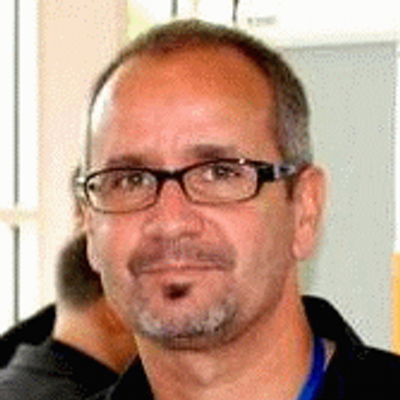
\includegraphics[width=0.35\linewidth]{Bilder/erich.png}
		\label{Erich Gamma}
		\quelle{siehe Fußnote\textsuperscript{1}}
	\end{center}
\end{floatingfigure}
\footnotetext[1]{$https://www.microsoft.com/italy/futuredecoded/$}
Erich Gamma wurde am 13. März 1961 in Zürich geboren und ist ein vergleichsweise sehr junger Pionier der Informatik. Er promovierte an der Universität Zürich in Informatik. Danach arbeitete er zunächst als Software-Ingenieur bei \textit{UBILAB}, einem Forschungslabor der \textit{Schweizerischen Bankgesellschaft} (heute \textit{UBS}) und anschließend bei \textit{Taligent}. Bekannt wurde er vor allem als Mitautor des Buches \textit{Design Patterns – Elements of Reusable Object-Oriented Software} \cite{gamma2004}. Das Buch entstand im Zuge seiner Dissertation gemeinsam mit Richard Helm, Ralph Johnson und John Vlissides. Vgl. \cite{ErichGammaWikiDe} \\ \\
Der Titel des Buches wurde in einiger Hinsicht als zu lang erachtet, deshalb wurde der kurze und prägnante Titel: Das Buch der Viererbande (engl.: Gang of Four, kurz: GoF) als Synonym etabliert vgl. \cite{GangOfFour}. Zusammen mit allen Mitglieder der \textit{GoF} erhielt er 2006 den Dahl-Nygaard-Preis, welcher für herausragende berufliche Leistungen im Bereich der Softwareentwicklung von der \textit{Association Internationale pour les Technologies Objets} vergeben wird vgl. \cite{Dahl-Nygaard-Preis}. \\ \\
Gamma war Initiator der offenen Entwicklungsumgebung Eclipse und hat deren Entwicklung ursprünglich geleitet. Außerdem war er einer der Hauptentwickler von \textit{ET++}, einer portablen \textit{C++}-Klassenbibliothek für interaktive grafische Anwendungen. Er war als Distinguished Engineer bei \textit{Rational Software}, eingestellt. \textit{Rational Software} ist eine Abteilung der \textit{IBM Software Group} in Zürich, welche sich schwerpunktmäßig mit System-, und Analysedesign beschäftigt. Er arbeitete dort am Projekt \textit{Jazz / Rational Team Concert}. Relativ überraschend wechselte er im August 2011 zur Microsoft Corporation für die er wieder als Distinguished Engineer tätig ist. Er leitet dort bis heute ein Team, das unterstützend an der Produktion der\textit{ Microsoft}-Entwicklungsumgebung \textit{Microsoft Visual Studio} mitwirkt. Vgl. \cite{ErichGammaWikiDe}

\chapter{Historische Leistung: Design Patterns}\label{se:Historische Leistung: Design Patterns}
Die deutsche Bezeichnung von Design Patterns ist Entwurfs Muster. Ein Muster ist im Allgemeinen eine gleichbleibende Struktur, in einer sich wiederholenden Sache. Da Muster auch wiederkehrende Denk- oder Verhaltensweisen sein können, ist die Bezeichnung Design Patterns treffend, denn sie bieten immer gleich bleibende Lösungsstrukturen für verschiedene Problemtypen im objektorierntierten Softwareentwurf.
\\ \\
Die Idee von Mustern wurde schon vor der Software Entwicklung in anderen Disziplinen als äußerst nützlich erkannt. Der 1939 in Wien geborene Architekt \mbox{Christopher} \mbox{Alexander} begann bereits 1975 mit der Veröffentlichung seiner Buchtrilogie: \textit{A Pattern Language} \cite{Alexander1979}, \textit{A Timeless Way of Building} \cite{Alexander1977} und \textit{The Oregon Experiment} \cite{Alexander1975}. Damit legte er lange vor der digitalen Revolution den Grundstein für eine allgemeine Definition von Mustern. Seine Werke stellen einen allgemeinen Ansatz zur Beschreibung von Mustern vor, konzentrieren sich aber im Konkreten auf Architektur und Stadtplanung. Auf die Arbeit von Christopher Alexander soll in Kapitel \ref{Muster} näher eingegangen werden.

\section{Motivation}\label{se:Motivation}

Ein großes Ziel der objektorientierten Softwareentwicklung ist die Erzeugung von wiederverwendbaren Teilen. Vor Gammas Arbeit\footnote{Hier und im Folgenden wird häufig von \glqq Gammas Arbeit\grqq{} gesprochen. Das kann den Eindruck erwecken, dass es sich um seinen alleinigen Verdienst handle. Natürlich ist in diesem Zusammenhang immer die Gesamtleistung aller Autoren des Buches \textit{Design Patterns – Elements of Reusable Object-Oriented Software} \cite{gamma2004} gemeint.} war der Design-Teil davon aber meistens ausgegrenzt. Es gab einfach kein universelles Werkzeug, um Designs wiederverwendbar zu machen.
\\ \\
Einen von Anfang an wiederverwendbaren und flexiblen Entwurf zu erstellen, kann sehr schwierig sein. Ein häufiges Abändern oder Revidieren von Entwürfen ist die Folge. Erich Gamma hat hier ein wichtiges Problem erkannt. Er sah die Tendenz, dass wiederkehrende Probleme immer wieder von Grund auf neu angegangen wurden. Das kostet Zeit und schafft viel Raum für Fehler. Vgl. \cite[S. 1]{gamma2004}
\\ \\
Erich Gamma wollte die Vorteile von Mustern auf den großen Bereich des objektorientierten Software Entwurfs ausweiten und adaptierte die Idee in diesen Bereich.

\section{Lösungsansatz}\label{se:Lösungsansatz}

Die Lösung des Problems ist ebenso einfach wie genial. Wurde ein Problem eines bestimmten Typs bereits einmal gelöst, kann das Konzept der Lösung in den meisten Fällen auch auf ähnliche Probleme angewandt werden.
\\ \\
Verschiedene Probleme erfordern verschiedene konkrete Lösungen, auch wenn sich die Art des Problems gleicht. Design Patterns abstrahieren Lösungen zu wiederkehrenden Problemen, um sie universell einsetzbar zu machen. Die konkreten Umsetzungen eines Musters können (und müssen) sich daher unterscheiden, jedoch teilt jede Umsetzung die Herangehensweise des zu Grunde liegenden abstrakt definierten Musters.
\\ \\
Als Grundlage für Design Patterns mussten einige Bestandteile von objektorientierten Softwaresystemen klar definiert werden. Zum Beispiel alle relevanten Objekte, Klassen und ihre Schnittstellen, Vererbungshierarchien oder Beziehungen zwischen den beteiligten Objekten und Klassen. Vgl. \cite[S. 1]{gamma2004}

\chapter{Design Patterns im Detail}\label{se:Design Patterns im Detail}
Der Unterschied zu den von Christopher Alexander vorgestellten Mustern ist, dass es sich beim objektorientierten Entwurf eben nicht um Türen und Wände, sondern um Objekte und Schnittstellen handelt vgl. \cite[S. 3]{gamma2004}.
Aus der Architektursicht schließen Design Patterns die Lücke zwischen Klassenbibliotheken und Frameworks. Dabei haben sie weniger Architekturelemente als ein Framework, sind dabei aber auch abstrakter. Letzteres hat wiederum den Vorteil, dass sie nicht auf bestimmte Programmiersprachen beschränkt sind. \\ \\
Nach \cite[S. 4]{gamma2004} sind Design Patterns 

\begin{quote}
	\textit{\glqq Beschreibungen zusammenarbeitender Objekte und Klassen, die maßgeschneidert sind, um ein allgemeines Entwurfsproblem in einem bestimmten Kontext zu lösen\grqq.}
\end{quote} 
\smallskip
Ein Design Pattern besteht dabei aus drei grundlegenden Teilen vgl. \cite{Gamma1993}:
\begin{enumerate}
	\item Einer abstrakten Beschreibung eines Zusammenspiels von Klassen oder Objekten und ihrer Struktur.
	\item Das Problem im Entwurf, das von dieser abstrakten Struktur gelöst werden soll.
	\item Die Konsequenzen für die Systemarchitektur, wenn die abstrakte Struktur darauf angewandt wird.
\end{enumerate}	

\section{Beschreibung von Design Patterns}\label{se:Beschreibung von Design Patterns}
Um einen Entwurf wiederverwendbar zu machen, reicht es nicht aus, sich ausschließlich auf grafische Notationen zu verlassen. Diese sind zwar wichtig, sagen aber z.B. nichts über mögliche Alternativen oder Vor- und Nachteile aus. Gamma wählte deshalb für sein Buch ein einheitliches Schema zur Beschreibung von Patterns aus vgl. \cite[S. 8-10]{gamma2004}. \\ \\
\textbf{Mustername und Klassifizierung} \\
Soll knapp und präzise den wesentlichen Gehalt des Patterns vermitteln. \\ \\
\textbf{Zweck} \\
Was macht das Pattern? Welchen Grundprinzip folgt es und welchem Zweck dient es? \\ \\
\textbf{Auch bekannt als} \\
Gibt es andere Bezeichnungen für dieses Pattern? \\ \\
\textbf{Motivation} \\
Beschreibt ein mögliches Szenario für den Einsatz dieses Patterns, also welches Entwurfsproblem adressiert wird. \\ \\
\textbf{Anwendbarkeit} \\
In welchen Problemsituationen kann dieses Pattern sinnvoll eingesetzt werden? Dieser Abschnitt hilft dem Entwickler dabei, solche Situationen zu identifizieren. \\ \\
\textbf{Struktur} \\
Hier findet die grafische Repräsentation der beteiligten Klassen und Objekte und deren Zusammenspiel in Form von Struktur-, und Interaktionsdiagrammen ihren Platz. \\ \\
\textbf{Teilnehmer} \\
Beschreibt teilnehmende Klassen und Objekte sowie deren Abhängigkeiten. \\ \\
\textbf{Interaktionen} \\
Wie arbeiten die Teilnehmer zusammen, um das Problem zu lösen? \\ \\
\textbf{Konsequenzen} \\
Diskutiert Vor- und Nachteile und beschreibt was von diesem Pattern zu erwarten ist. Außerdem wird hier angegeben, welche Teile der Systemstruktur unabhängig voneinander variiert werden können. \\ \\
\textbf{Implementierung} \\
Adressiert Fallen, Tips oder Techniken zur Implementierung des Patterns. \\ \\
\textbf{Beispielcode} \\
Codefragmente von \textit{C++} oder \textit{Smalltalk} zur Veranschaulichung. \\ \\
\textbf{Bekannte Verwendungen} \\
Zeigt Beispiele für das Pattern auf, die in echten Systemen zu finden sind. \\ \\
\textbf{Verwandte Muster} \\
Diskutiert relevante Unterschiede zu ähnlichen Patterns und gibt an, mit welchen anderen Patterns eine gute Harmonie.
\section{Klassifizierung von Design Patterns}\label{se:Klassifizierung}

\begin{table}[H]
	\caption{Ketegorisierung von Mustern nach ihrer Aufgabe. Vgl. \cite[S. 14]{gamma2004}}\label{ta:Klassifizierung}
	\begin{center}
		\begin{tabular}{|l|l|l|}
			\hline
			\bf Erzeugungsmuster   & \bf Strukturmuster                & \bf Verhaltensmuster       \\
			\hline
			\textit{Fabrikmethode} & \textit{Adapter (klassenbaisert)} & \textit{Interpreter}       \\
			Abstrakte Fabrik       & Adapter                           & \textit{Schablonenmethode} \\
			Erbauer                & Brücke                           & Befehl                     \\
			Prototyp               & Dekorierer                        & Beobachter                 \\
			Singelton              & Fassade                           & Besucher                   \\
			                       & Fliegengewicht                    & Iterator                   \\
			                       & Kompositum                        & Memento                    \\
			                       & Proxy                             & Strategie                  \\
			                       &                                   & Vermittler                 \\
			                       &                                   & Zustand                    \\
			                       &                                   & Zuständigkeitskette       \\
			\hline
		\end{tabular}
	\end{center}
	\begin{center}
		\small{\textit{Klassenbasierte Muster sind jeweils kursiv gedruckt.}}
	\end{center}
\end{table}

Muster können anhand ihrer Aufgabe unterteilt werden (siehe Tabelle \ref{ta:Klassifizierung}). Diese kann \textbf{ erzeugend},\textbf{ strukturorientiert} oder \textbf{verhaltensorientiert} sein. Ein weiteres Kriterium ist der Gültigkeitsbereich eines Musters. Dieser sagt aus, ob sich ein Muster primär auf Objekte oder auf Klassen bezieht.
Dieses Kapitel befasst sich primär mit der Klassifizierung nach der Muster Aufgabe. Diese sollen jeweils beschrieben und im folgenden Kapitel jeweils mit einem typischen Beispielmuster vorgestellt werden. 
\\ \\
Zu erwähnen bleibt trotzdem, dass sich Muster auch auf andere Weisen klassifizieren lassen. Beispielsweise können oft zusammen benutzte Muster oder Alternativ-Muster zu einem gegebenen Problem gebündelt werden. Vgl. \cite[S. 14]{gamma2004}

\subsection{Erzeugungsmuster}\label{se:Erzeugungsmuster}

Erzeugungsmuster dienen, wie der Name erahnen lässt, zur Erzeugung von Objekten. Man verwendet sie, um das Wissen der im System verwendeten Klassen zu kapseln. Die Anwendung soll nur den für sie relevanten Anteil der erzeugten Objekte kennen, nämlich den, der über die Erzeuger-Schnittstelle nach außen sichtbar ist. Über Produktionsobjekte lassen sich statisch oder zur Laufzeit Produktionen konfigurieren und somit beliebig komplizierte Erzeugungsprozesse nach außen hin verstecken. Das System wird dadurch unabhängig davon, wie es seine Objekte erzeugt, zusammensetzt oder repräsentiert. 
\\
Erzeugungsmuster werden dann besonders hilfreich, wenn Abhängigkeiten zwischen Klassen vor allem durch Kompositionen und nicht durch Vererbung definiert sind. Vgl. \cite[S. 101]{gamma2004}

\subsection{Strukturmuster}\label{se:Strukturmuster}

Strukturmuster stellen Beziehungen zwischen Klassen und Objekten her und schaffen so größere Gesamtstrukturen. Es gibt sowohl objekt-, als auch klassenbasierte Strukturmuster, die sich in ihren Konzepten unterscheiden. Objektbasierte Strukturmuster führen Objekte zusammen, klassenbasierte Strukturmuster nutzen Vererbung um Schnittstellen und Implementierungen zusammenzuführen. Ziel ist wiederum die Entkopplung der beteiligten Elemente.

\subsection{Verhaltensmuster}\label{se:Verhaltensmuster}

Verhaltensmuster befassen sich mit der Problematik, Interaktionen zwischen Objekten zu organisieren. Dabei werden auch komplexe Kontrollflüsse beschrieben. \\
Klassenbasierte Verhaltensmuster greifen auf Vererbung zurück, um Funktionalitäten an andere Klassen weiterzugeben. \\
Objektbasierte Verhaltensmuster verwenden stattdessen Objektkomposition (z.B. durch Aggregation). Viele von Erich Gamma vorgestellten objektbasierte Verhaltensmuster beschreiben, wie Gruppen von Objekten an einer Aufgabe beteiligt sind, die keines der teilnehmenden Objekte alleine lösen könnte. Ein Muster muss somit die Abhängigkeiten der einzelnen Objekte auf sinnvolle Weise festlegen. Vgl. \cite[S. 271]{gamma2004}

\section{Beispiele}
In diesem Kapitel wird für jede der drei Klassifizierungsansätzen ein typisches von Gamma vorgestelltes Beispielmuster im Detail beschrieben.

\subsection{Beispiel für Erzeugungsmuster: Abstrakte Fabrik}

Ein klassisches Erzeugungsmuster ist die Abstrakte Fabrik. Zweck des Musters ist es, Objekte zu erzeugen, die verwandt oder voneinander abhängig sind. Dazu bietet die Fabrik eine Schnittstelle an, ohne die konkreten Klassen zu benennen. Vgl. \cite[S. 107]{gamma2004}

\begin{figure}[H]
	\centering
	\includegraphics[width=\ScaleIfNeeded]{Bilder/Abstrakte_Fabrik.png}
	\caption{Abstrakte Fabrik Muster}
	\quelle{ Vgl. \cite[S. 109]{gamma2004}}
	\label{fig:Abstrakte_Fabrik}
\end{figure}
\ \\
Abbildung \ref{fig:Abstrakte_Fabrik} zeigt das Konzept des Musters. In diesem Beispiel gibt es zwei abstrakte Produkte, mit wiederum jeweils zwei konkreten Ausprägungen. Der Klient kennt nur die abstrakte Fabrik, die hier die Schnittstelle zweier konkreter Fabriken ist, sowie die beiden abstrakten Produkte. Und genau so findet die Entkopplung statt; Der Klient manipuliert Objekte nur über ihre abstrakten Schnittstellen. Die Interaktion mit Produkten findet somit über Schnittstellen statt, konkrete Produkte muss er nicht kennen. Konkrete Fabriken werden normalerweise zur Laufzeit erzeugt. Diese muss der Klient natürlich kennen, damit er verschiedene Produktobjekte erzeugen kann. \\
Dieses Muster bietet sich vor Allem dann an, wenn zu erwarten ist, dass zu einem späteren Zeitpunkt keine weiteren Produkte mehr hinzukommen. Weil die Schnittstelle der Fabrik festlegt, welche Produkte hergestellt werden können, müssten diese um das neue Produkt erweitert werden. Das hat die Folge, dass auch alle konkreten Fabriken überarbeitet werden müssen. Eine Erweiterung innerhalb der Produktfamilien kann sich also als schwierig herausstellen. Vgl. \cite[S. 109-111]{gamma2004}

\subsection{Beispiel für Strukturmuster: Dekorierer}

Manchmal kann es sinnvoll sein, die Funktionalitäten eines Objekts zu erweitern, ohne dabei die Klasse zu verändern. Eine Lösung dafür wäre Vererbung. Vererbung stellt sich in diesem Fall aber als unflexibel heraus, weil die Auswahl der vererbenden Klasse statisch, also nicht beliebig austauschbar ist. Vlg. \cite[S. 199]{gamma2004}
\\ \\
Als Lösung für dieses Problem bietet sich ein häufig eingesetztes objektbasiertes Strukturmuster, nämlich das Dekorierer Muster an. Zweck des Musters ist es, Klassen dynamisch mit zusätzlichen Informationen und Funktionalitäten anzureichern. Das Muster stellt in vielen Fällen eine flexible Alternative zur Vererbung dar. Vgl. \cite[S. 199 ]{gamma2004}

\begin{figure}[H]
	\centering
	\includegraphics[width=0.75\linewidth]{Bilder/Dekorierer.png}
	\caption{Dekorierer Muster}
	\quelle{ Vgl. \cite[S. 201]{gamma2004}}
	\label{fig:Dekorierer}
\end{figure}

\begin{figure}[H]
	\centering
	\includegraphics[width=0.8\linewidth]{Bilder/dekorierer_2.png}
	\caption{Beispiel einer dekorierten Komponente}
	\quelle{Vgl. \cite[S. 205]{gamma2004}} 
	\label{fig:Beispiel einer dekorierten Komponente}
\end{figure}
\ \\
Der Aufbau des Musters ist in Abbildung \ref{fig:Dekorierer} dargestellt. Jede konkrete Komponente und jeder Dekorierer erben von einer abstrakten Basis-Komponente. Die Grundidee des Musters zeigt sich im Dekorierer. Er hält eine weitere Komponente vor, die wiederum eine konkrete Komponente oder aber ein weiterer Dekorierer sein kann. So können beliebig lange Ketten gebildet werden (siehe Abbildung \ref{fig:Beispiel einer dekorierten Komponente}). Bestehende Strukturen werden mit neuen Informationen \glqq dekoriert\grqq. Dekorierer wiederum können verschiedene konkrete Ausprägungen besitzen, die zum Beispiel zusätzliche Zustände oder weitere Funktionen hinzufügen.
\\ \\
Dieses Muster ermöglicht es außerdem, dass Objekte erst zur Laufzeit mit Informationen angereichert werden können. Im direkten Vergleich mit klassischer Mehrfachvererbung, bietet dieses Muster eine deutlich größere Flexibilität und hält dabei die Komplexität des Systems im Verhältnis klein. Bei einer äquivalenten Lösung mittels Mehrfachvererbung, muss für jede zusätzliche Funktionalität eine weitere Klasse erzeugt werden. Ein mehrfaches Hinzufügen der gleichen Information ist ebenso möglich, wie ein Mischen von Funktionen, was wiederum mit Mehrfachvererbung schwer lösbar ist und bestenfalls als fehleranfällig bezeichnet werden kann. Vgl. \cite[S. 203]{gamma2004}
\\ \\
Es macht Sinn die Basiskomponente nicht mit Funktionalität zu überfrachten. Sie sollte nur die Funktionalität bieten, die alle (auch in Zukunft hinzukommenden) Komponenten besitzen sollen. Individualität der Komponenten wird durch weitere konkrete Dekorierer ermöglicht. Vgl. \cite[S. 203 - 204]{gamma2004}

\subsection{Beispiel für Verhaltensmuster: Strategie}
Will man mehrere Algorithmen zu einer bestimmten Problemstellung kapseln und austauschbar machen, bietet sich dafür das objektbasierte Verhaltensmuster Strategie an.

\begin{figure}[H]
	\centering
	\includegraphics[width=\ScaleIfNeeded]{Bilder/Strategie.png}
	\caption{Strategie Muster}
	\quelle{Vgl. \cite[S. 375]{gamma2004}} 
	\label{fig:Strategie}
\end{figure}
\ \\
Das Konzept des Musters ist sehr einfach und lässt sich schnell umsetzen. Ein Beispiel mit drei konkreten Algorithmen ist in Abbildung \ref{fig:Strategie} zu sehen. Der Kontext, der die Strategie nach außen an seine Klienten anbietet, hält ein Objekt des Typs Strategie vor und ist in Besitz alle für die Algorithmen notwendigen Daten. Eine Strategie ist wiederum die Schnittstelle für konkrete Strategien, welche wiederum jeweils eine andere (austauschbare) Variante eines Algorithmus implementieren. Damit wird eine Entkopplung der Algorithmen und der Klassen die sie benötigen hergestellt. Natürlich muss dafür der konkrete Algorithmus für die Auswahl, bei der anwendenden Klasse bekannt sein. Eine Möglichkeit die Algorithmen mit Eingabedaten zu versorgen wäre, indem sich der Kontext selbst der Strategie übergibt. Die Strategie kann dann je nach Bedarf selbst auf die von ihr benötigten Daten zurückgreifen.

\chapter{Herkunft und Reichweite}\label{Muster}
Das Konzept der Muster wurde vor allem von Christopher Alexander geprägt. Seine Bücher zu Mustern in Gebäude und Städtebau können heute als Klassiker bezeichnet werden, die nach wie vor große Bedeutung tragen. Muster haben sich in vielen anderen Bereichen, auch abseits der Architektur, durchgesetzt. Dieses Kapitel soll die Idee Alexanders vorstellen, ihre Umsetzung in der Gebäude-, und Städtearchitektur kurz beleuchten und als Beispiel für die Reichweite seiner Werke das vergleichsweise neue Konzept der bekannten Anti-Patterns vermitteln.

\section{Die Idee des Musters nach Christopher Alexander}
\cite{Alexander1977}

\subsection{Muster in der Gebäude- und Stadtarchitektur}

\subsection{Unterschiede zu Gammas Arbeit}
Auch wenn das von Christopher Alexander etablierte Konzept der Muster einen großen Einfluß auf viele andere Bereiche hatte, finden sich insbesondere zu Gammas Veröffentlichungen einige Unterschiede: Vgl. \cite[S. 438 - 439]{gamma2004}

\begin{enumerate} 
\item Alexander beschäftigt sich mit Gebäuden und Städten, die von Menschen bereits seit Tausenden von Jahren gebaut werden. Deshalb existierten viele Beispiele, auf die er sich beziehen konnte. Softwaresysteme wurden zur Zeit von Gammas Veröffentlichungen erst seit relativ kurzer Zeit konstruiert und nur wenige davon konnten damals als klassisch bezeichnet werden.
\item Außerdem gibt Alexander eine Anwendungsreihenfolge seiner Muster an, Gamma macht das nicht.
\item Ein weiterer Unterschied ist die Herangehensweise. Alexander betont die von ihm adressierten Probleme, Gamma konzentriert sich dagegen mehr auf Lösungen.
\item Der letzte wirklich große Unterschied zu Gamma ist, dass Alexander behauptet, dass seine Muster vollständige Gebäude erzeugen können. Gamma erhebt nicht den Anspruch darauf, dass seine Muster vollständige Programme erzeugen können.
\end{enumerate}

\section{Anti-Pattern}
Anti-Pattern drehen das Vorgehen für den Entwickler um, indem sie zeigen, wie man es am besten nicht machen sollte. Sie bilden somit das genaue Gegenstück zu den Mustern. Diese Pattern beschränken sich keineswegs nur auf die Entwicklung von Software, sondern haben Ausläufer in viele verschiedene Bereiche, darunter z.B. Architektur, Organisation oder Management. \cite{AntiPatternsCatalog}

\chapter{Nutzen von Design Patterns heute}\label{se:Design Patterns heute}

Design Patterns haben bis heute nichts von ihrer Relevanz verloren. Das Gegenteil ist der Fall, sie sind aus dem objektorientierten Entwurf nicht mehr weg zu denken. Design Patterns liefern sie nach wie vor viele Vorteile vgl. \cite{Gamma1993}:
\begin{itemize}
	\item Für Entwickler sind sie ein wichtiges Werkzeug, das ihnen hilft Entwürfe zu kommunizieren oder Entwurfs-Alternativen zu finden.
	\item Sie reduzieren die Systemkomplexität, indem sie Abstraktionen definieren, die über Klassen und Instanzen stehen.
	\item Sie bilden eine Basis von erprobten Lösungsschemata, die es dem Entwickler auch heute noch sehr hilft, wiederverwendbare Software zu produzieren.
	\item Sie destillieren erprobte Erkenntnisse des Softwareentwurfs von erfahrenen Entwicklern und bilden so Bausteine, die es ermöglichen, komplexe Gesamtsysteme zu erzeugen.
	\item Sie helfen dem Entwickler die Einarbeitungszeit in existierende Klassenbibliotheken zu reduzieren. Sind die Design Patterns innerhalb der Klassenbibliothek erst einmal verstanden, hilft sie dabei andere Bibliotheken schneller zu verstehen.
	\item Design Patterns unterstützen den Entwickler dabei, Reorganisationen oder Refaktorisierungen einfacher und schneller durchzuführen.
\end{itemize}
   

\newpage
\bibliography{literatur}

\end{document}